\documentclass[12pt,a4paper]{report}
\usepackage[latin1]{inputenc}
\usepackage{amsmath}
\usepackage{amsfonts}
\usepackage{subfigure}
\usepackage{amssymb}
\usepackage[pdftex]{graphicx}
\begin{document}

\noindent
{\bf Fully Connected Results on CIFAR-10} \\ 

A network consisting of 512 features, followed by pooling with overlap in 1-D code space (509 pooled features after pooling with no wrap around), was trained on about 175,000 frames collected from YouTube.
The RGB frames were down-sampled and resized to 32x32. \\ 

The unsupervised network is: Linear$\rightarrow$Threshold $\rightarrow$L2-Pooling.
Two unsupervised learning algorithms are compared here: (1) group sparsity (i.e. L1-Penalty after pooling), (2) L1 penalty before pooling and L1-slow feature penalty after pooling. 
Six models were trained using Group Sparsity and six using the Slow Feature penalty (total of 12 models).  
A comparison is also made to 10 randomly generated features. \\

The learned features were used to initialize the first linear layer of a fully connected classifier network: Linear$\rightarrow$Threshold$\rightarrow$L2-Pooling$\rightarrow$Linear$\rightarrow$LogSoftMax. \\

The classification results were obtained as follows: (1) 40,000 samples for training, (2) 10,000 for validation, (3) 10,000 for test. Over 30 training epochs choose the error  corresponding to the smallest validation error. \\

Since these networks have relatively few features for fully connected features, the bottom line results are quite poor compared to the "state of the art". The best test error was 58.42\%. 
The parameter settings using were just best guesses. I should repeat these experiment with a smaller group sparsity penalty because the best error achieved using group sparsity is the one corresponding to th smallest regularization strength. \\ 

In general it is naive to expect to resolve the differences between these two pre-training methods in such a small setting (too few features, too little video data, etc), although a small difference can be seen already. 

\newpage 
The table below summarizes the strength of the regularization used to pre-train the models.  
\begin{center}
    \begin{tabular}{| l | l | l |}
    \hline
   Model Number &  Group Sparsity & Slow Feature\\ \hline
    1&L1=0.5&L1=2.0,SF=1.0 \\ 
    2&L1=1.0&L1=0.0,SF=2.0 \\
    3&L1=1.5&L1=1.0,SF=2.0 \\    
    4&L1=2.0&L1=2.0,SF=2.0 \\      
	5&L1=2.5&L1=0.5,SF=3.0 \\    
	6&L1=3.0&L1=1.0,SF=3.0 \\ 
    \hline
    \end{tabular}
\end{center}

\begin{figure}[ht]
\centering 
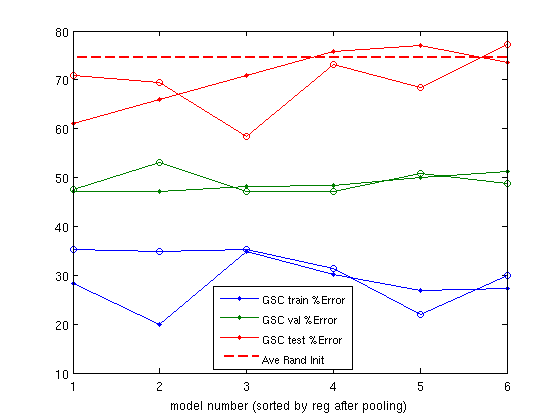
\includegraphics[scale=0.8]{class_graph.png}
\caption{Classification ERROR on CIFAR-10. Plots with \emph{DOTS} correspond classifiers initialized with features learned using Group Sparsity, \emph{CIRCLES} correspond to classifiers initialized using Slow Features. The dashed line represents the average (averaged over 10 random initializations) test-set error achieved using randomly initialized features.}  
\end{figure} 

\begin{figure}
\centering 
\begin{subfigure}
		\centering 
		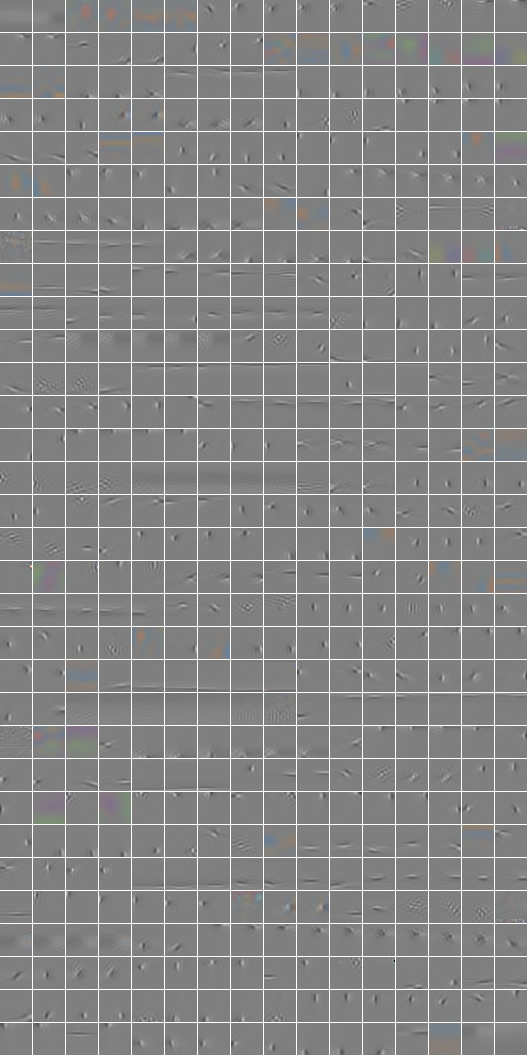
\includegraphics[width=3.5cm, height=10cm]{./decoder_images/gsc_05.png}
	%	\caption{df}
    \end{subfigure} 
	\begin{subfigure}
		\centering 
		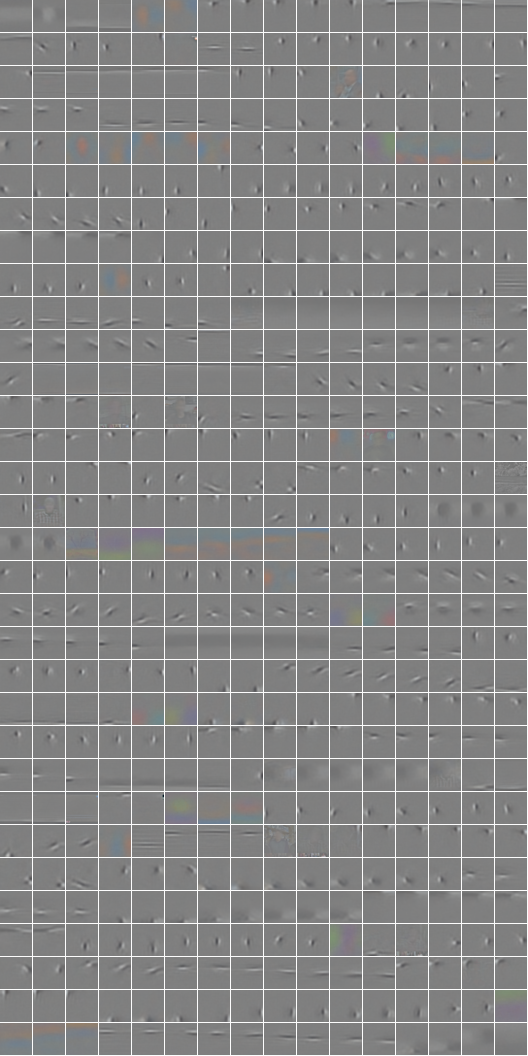
\includegraphics[width=3.5cm, height=10cm]{./decoder_images/gsc_10.png}
%		\caption{cfg}
	\end{subfigure} 
	\begin{subfigure}
		\centering 
		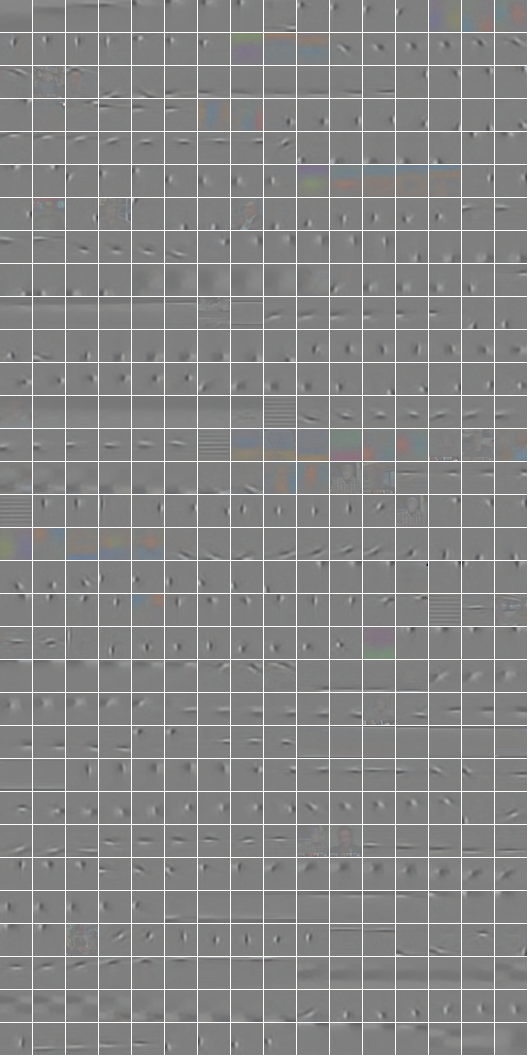
\includegraphics[width=3.5cm, height=10cm]{./decoder_images/gsc_15.png}
%		\caption{}
	\end{subfigure} \\
	\begin{subfigure}
		\centering 
		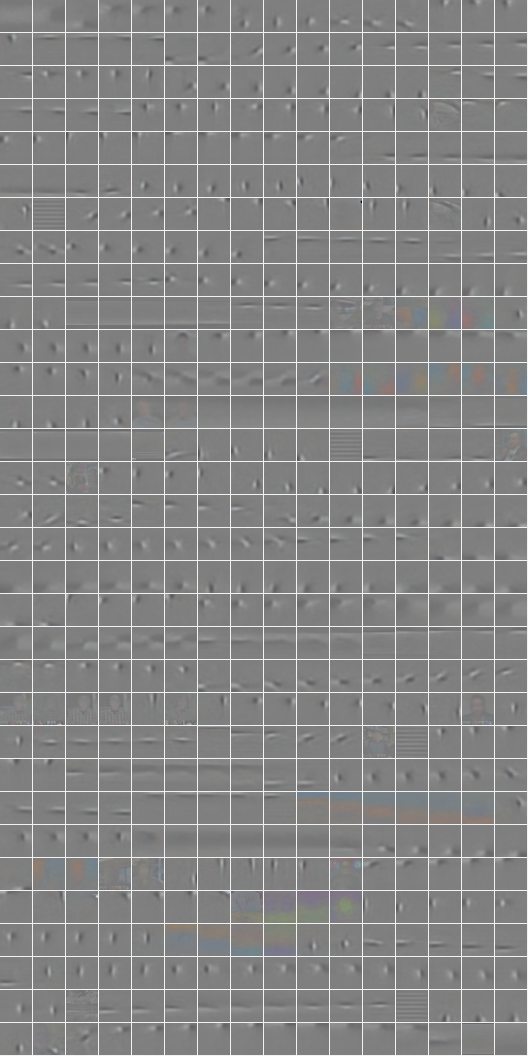
\includegraphics[width=3.5cm, height=10cm]{./decoder_images/gsc_20.png}
%		\caption{}
	\end{subfigure} 
	\begin{subfigure}
		\centering 
		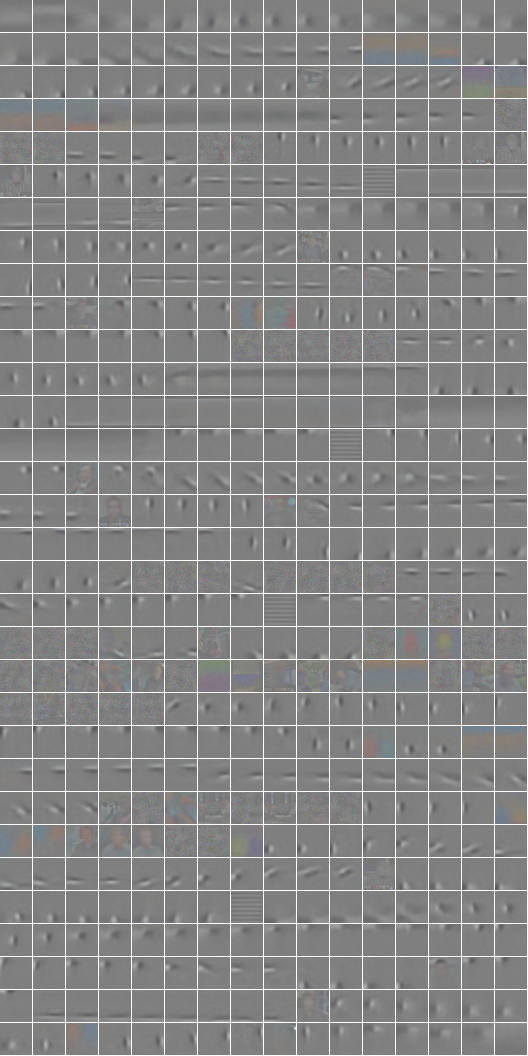
\includegraphics[width=3.5cm, height=10cm]{./decoder_images/gsc_25.png}
%		\caption{}
	\end{subfigure} 
	\begin{subfigure}
		\centering 
		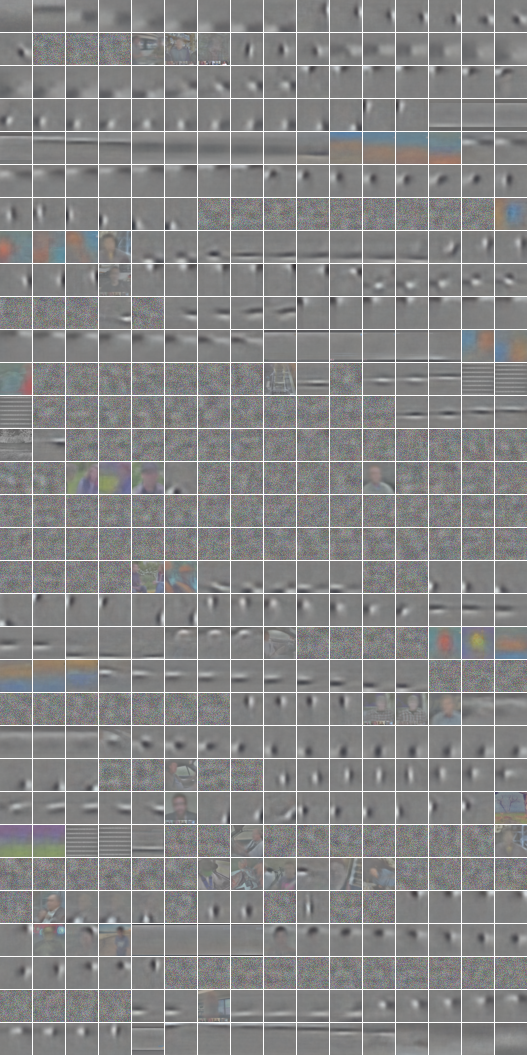
\includegraphics[width=3.5cm, height=10cm]{./decoder_images/gsc_30.png}
%		\caption{}
	\end{subfigure} 
%	\begin{subfigure}[b]{0.2\textwidth}
%		\centering 
%		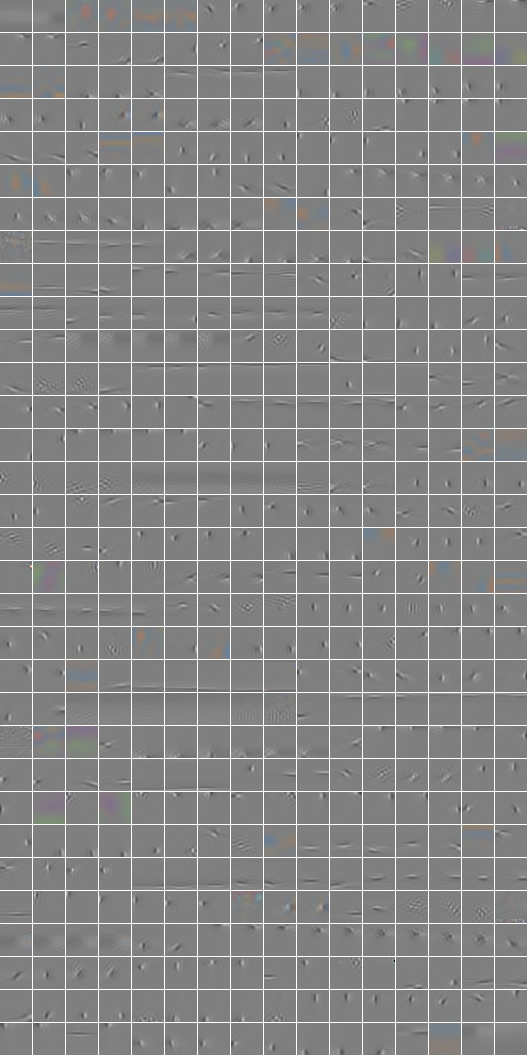
\includegraphics[width=2.5cm, height=10cm]{./decoder_images/gsc_05.png}
%		\caption{}
%	\end{subfigure} 
%	\begin{subfigure}[b]{0.2\textwidth}
%		\centering 
%		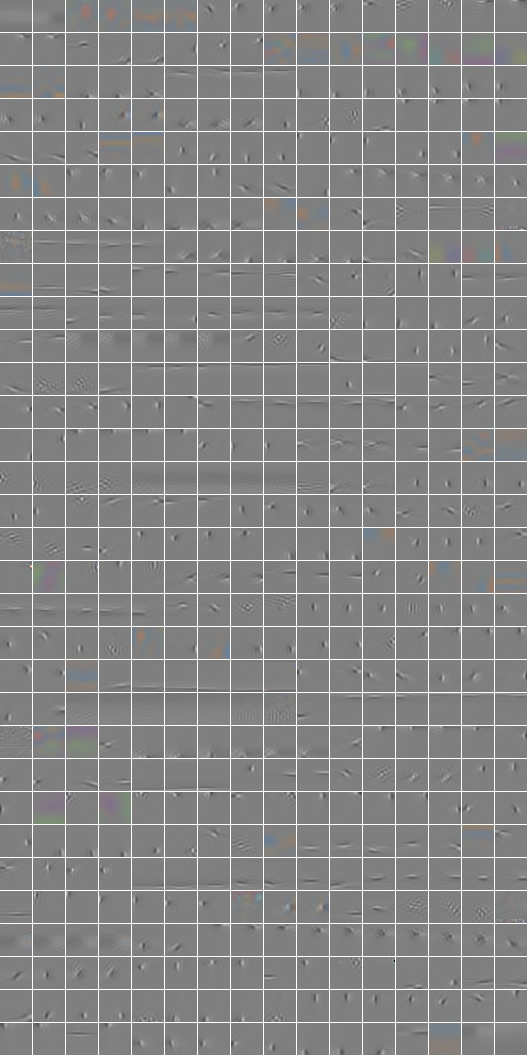
\includegraphics[width=2.5cm, height=10cm]{./decoder_images/gsc_05.png}
%		\caption{}
	%\end{subfigure} 
\caption{Features learned using Group Sparsity sorted by increasing slowness penalty (in order from top-left they models 1-6)} 
\end{figure} 
\newpage 

\begin{figure}[ht]
\centering 
\begin{subfigure}
		\centering 
		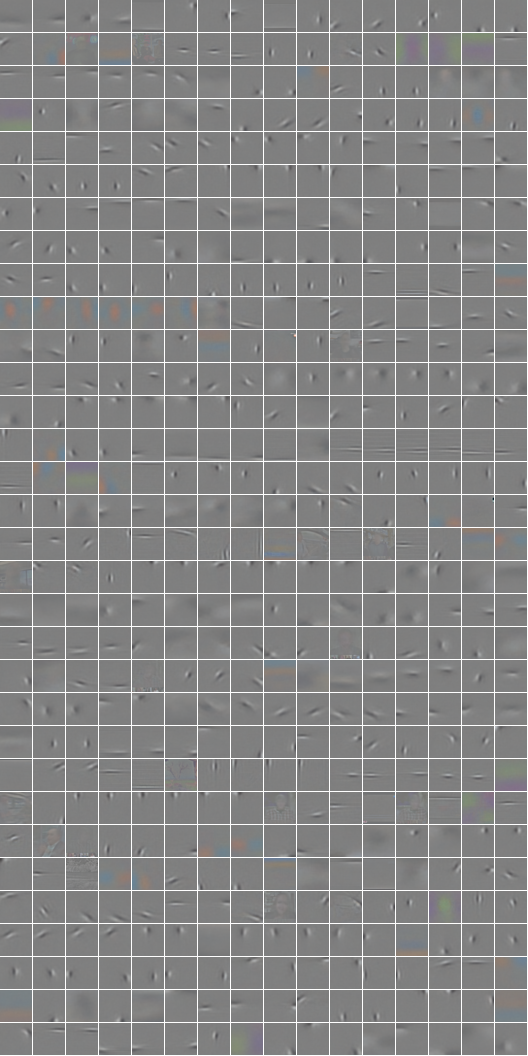
\includegraphics[width=3.5cm, height=10cm]{./decoder_images/sf_model1.png}
	%	\caption{df}
    \end{subfigure} 
	\begin{subfigure}
		\centering 
		
\includegraphics[width=3.5cm, height=10cm]{./decoder_images/sf_model2.png}
%		\caption{cfg}
	\end{subfigure} 
	\begin{subfigure}
		\centering 
		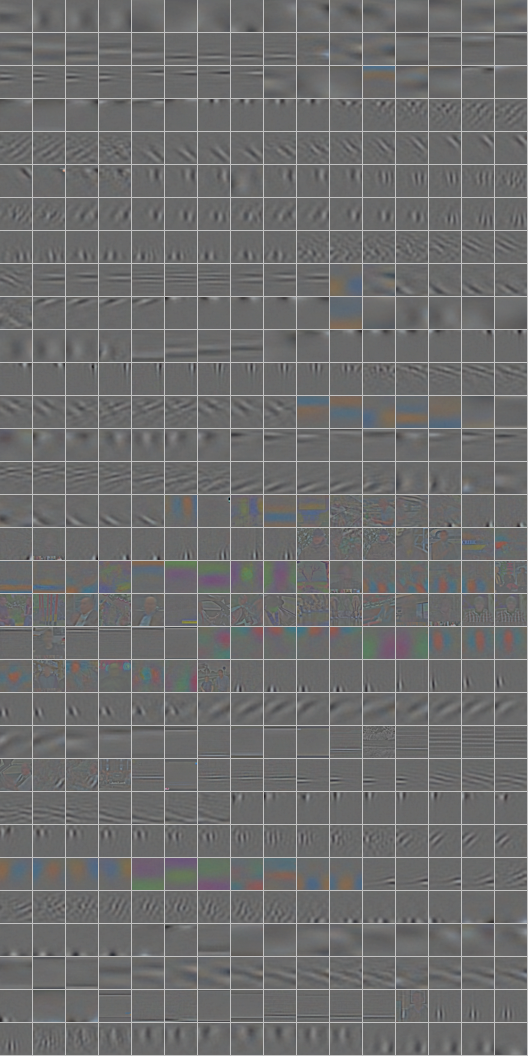
\includegraphics[width=3.5cm, height=10cm]{./decoder_images/sf_model3.png}
%		\caption{}
	\end{subfigure} \\
	\begin{subfigure}
		\centering 
		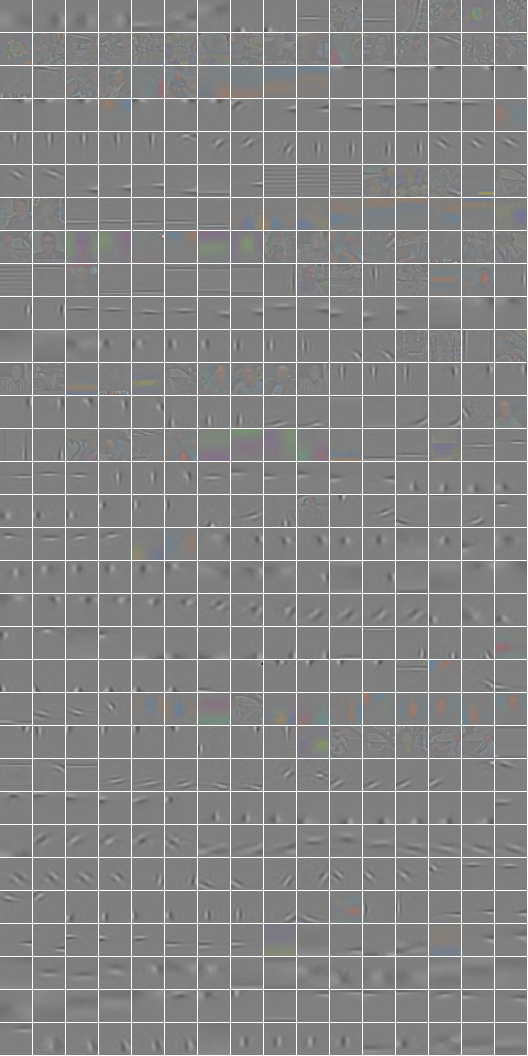
\includegraphics[width=3.5cm, height=10cm]{./decoder_images/sf_model4.png}
%		\caption{}
	\end{subfigure} 
	\begin{subfigure}
		\centering 
		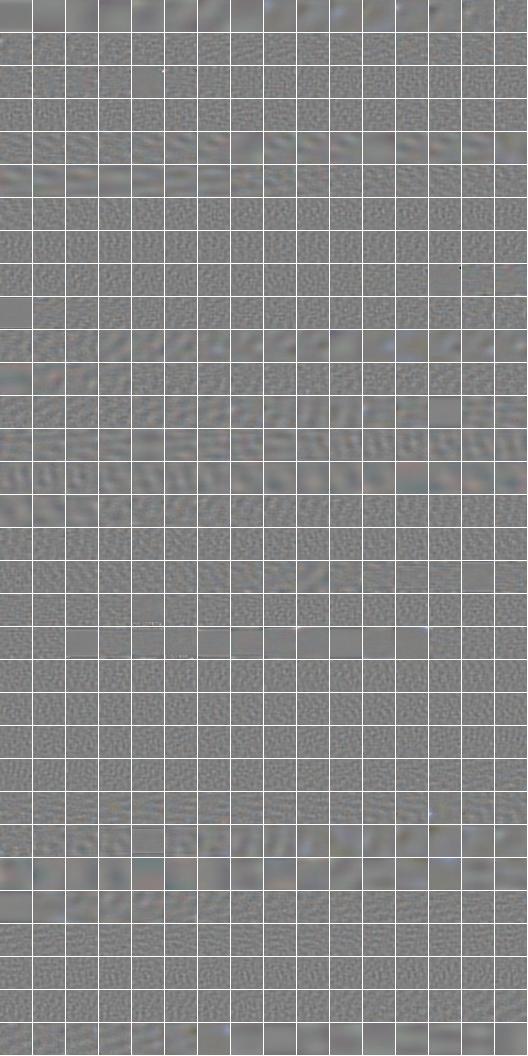
\includegraphics[width=3.5cm, height=10cm]{./decoder_images/sf_model5.png}
%		\caption{}
	\end{subfigure} 
	\begin{subfigure}
		\centering 
		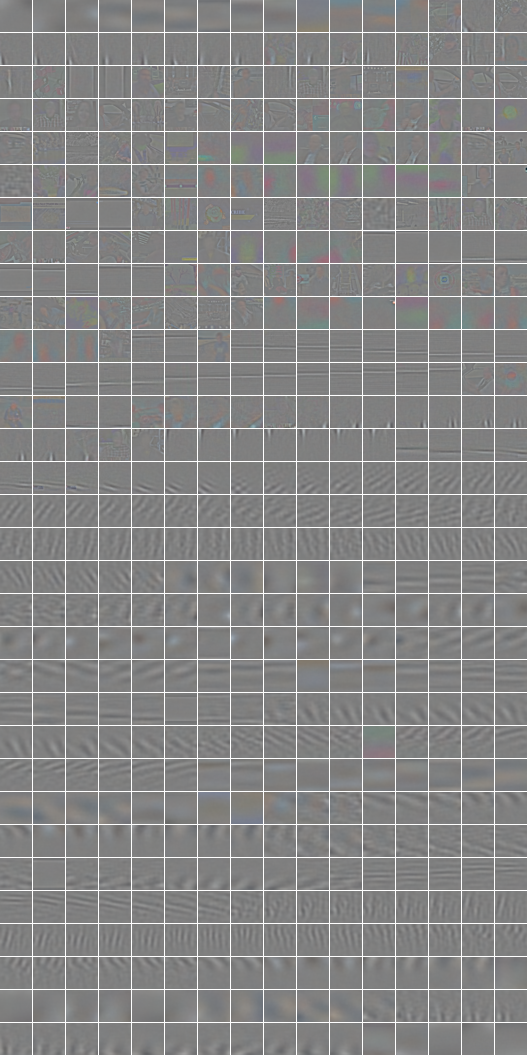
\includegraphics[width=3.5cm, height=10cm]{./decoder_images/sf_model6.png}
%		\caption{}
	\end{subfigure} 
%	\begin{subfigure}[b]{0.2\textwidth}
%		\centering 
%		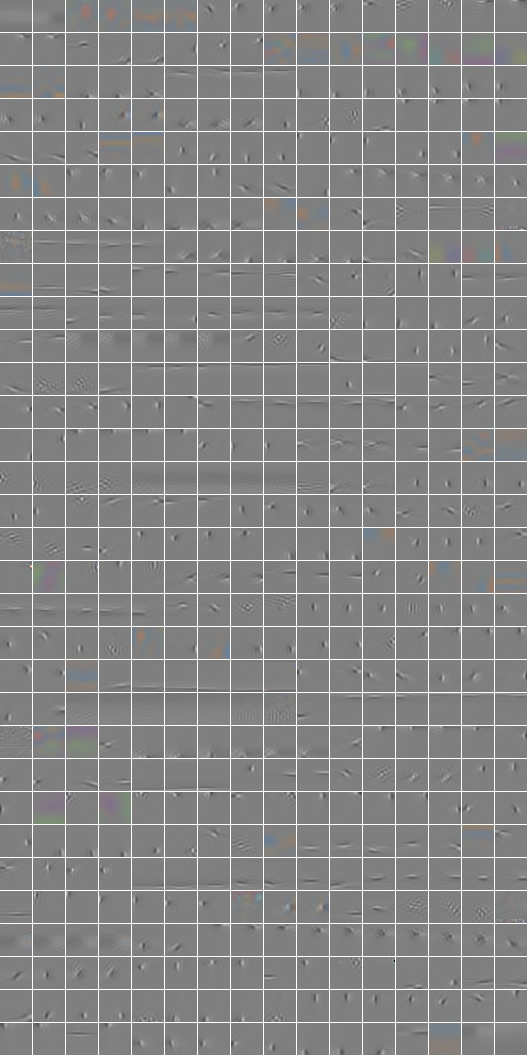
\includegraphics[width=2.5cm, height=10cm]{./decoder_images/gsc_05.png}
%		\caption{}
%	\end{subfigure} 
%	\begin{subfigure}[b]{0.2\textwidth}
%		\centering 
%		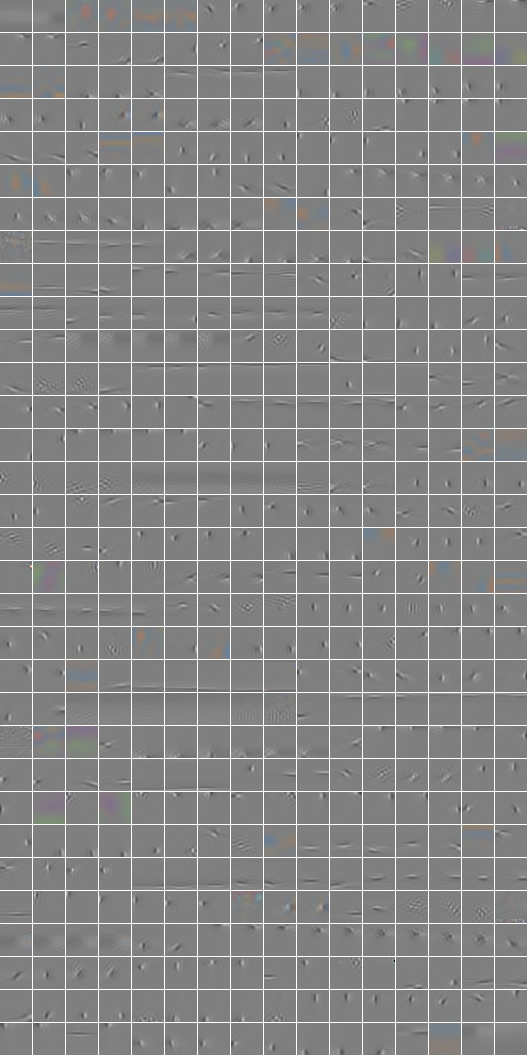
\includegraphics[width=2.5cm, height=10cm]{./decoder_images/gsc_05.png}
%		\caption{}
	%\end{subfigure} 
		\caption{Slow features sorted by increasing slowness penalty (in order from top-left they models 1-6)}

\end{figure} 

\end{document}